\section{Implementation: The Routing Sandbox}
\label{sec:sandbox_implementation}

In this section, we describe a prototype, the {\em routing sandbox}, that
incorporates BGP route prediction algorithms described in this chapter.
Our current prototype separates the computation of egress routers for a
given destination from the assignment of other routers to those egress
routers.   {\em This separation of functionality requires that $b_r \in
\gamma(E)$, which does not hold when {\em both} MED and route reflection are
used (as shown in Section~\ref{sec:rr_med}).}  
%We refer readers to our
%previous work, which discusses the design, implementation, and evaluation
%of the prototype implementation in more detail~\cite{Feamster2004}. 

\subsection{Design Overview}

We now highlight the high-level design of the prototype, shown in
Figure~\ref{fig:dataflow}.  We 
briefly describe the necessary inputs for driving the prototype, the
decomposition of functionality into three distinct modules and the
relationships of those modules to the algorithms described in this
chapter, and optimizations that reduce computational complexity.

\begin{figure}[h!]
\centering \epsfig{file=sandbox/figures/prototype_fig.eps, width=\linewidth}
\caption[Data flow in the prototype.]{Data flow in the prototype.  Fonts
  specify {\emc raw 
  inputs}, {\mfc input tables}, and {\dfc derived tables}.  In
  practice, operators might 
  collect raw inputs once a day.}
\label{fig:dataflow}
\end{figure}


%\subsubsection{Input data}
The prototype has three inputs:

\begin{itemize}
\item {\em BGP routing tables:}
The BGP tables for the eBGP-speaking routers provide the first stage of the
algorithm with a snapshot of the routes advertised by neighboring
ASes.  We ignore the router's current view of the best route and the
current setting of the local preference attribute, since these relate
to the existing network configuration rather than the scenarios we
might want to emulate.

\item {\em Router configuration files:} The configuration files are used
to (1)~determine the import policies (\ie, ``route maps'', as described
in Section~\ref{sec:configuration}) for each eBGP
session, (2)~determine the iBGP signaling graph, and (3)~compute the IGP
path costs between each pair of routers.  The import policies are used
to manipulate attributes of the eBGP routes in the first stage of the
algorithm, and the iBGP and IGP information are needed for the third
stage.

\item {\em BGP neighbor information:}
Because BGP route selection (Table~\ref{tab:background:decision})
depends on the router ID associated 
with the BGP session announcing the route, our algorithms require
knowing the router ID associated with each BGP session.  The second
stage uses the router IDs of the {\em eBGP\/} sessions, while the
third stage uses the router IDs for the {\em iBGP\/} sessions.
\end{itemize}
\noindent
%We emphasize several points with regard to the input data.  
We note that these inputs are easy to either obtain or approximate.
First, a
network operator can capture all of the necessary data with {\tt telnet} or
{\tt ssh} access to each router.  Second, many aspects of the input data do
not change very often; as such, the prototype is useful even if all of
the input data is collected infrequently (\eg, once a day).  Finally,
because certain inputs can be approximated (\eg, a BGP session's router
ID is typically the loopback IP address\footnote{A router's {\em loopback
address} is an IP address on the router that is reachable via any of
the router's interfaces.}
of the router on the opposite
end of the session), the prototype can be effective even with limited
input.


%\subsubsection{Prototype operation}  

The prototype uses a database back-end,
which provides efficient access to small subsets of the configuration
data and routes and also stores intermediate results, which allow us to
validate each part of the algorithm separately.
Figure~\ref{fig:dataflow} summarizes how the prototype uses the inputs
and intermediate results to generate a table of predicted routes.  The
three modules shown in Figure~2 correspond to the first two stages from
Section~\ref{sec:decompose}; assuming that $b_r \in \gamma(E)$ allows us
to break the second stage into two simpler modules.  The prototype
performs three operations:

{\em Applying import policy to eBGP-learned routes:} This operation
corresponds to the first step described in Section~\ref{sec:decompose}.
Each row of the {\mfc import} table specifies how a particular set of
rows in the {\mfc known routes} table should be modified; the prototype
performs the actual modifications on the {\dfc modified routes} table.
For each row in the {\mfc import} table, the first operation applies the
policy by (1)~finding the appropriate routes by selecting the set of
routes learned at the corresponding router on that BGP session that
match the specified AS path regular expression and (2)~setting the other
attributes (\eg, local preference) according to the values specified in
that row of the {\mfc import} table.

{\em Computing the egress routers for a destination:} This operation
generates the set of best eBGP-learned routes, $B$, using the
algorithm from Section~\ref{sec:fm_med},
corresponding to the first half of stage~2 in
Section~\ref{sec:decompose}.  
%(As long as $b_r \in \gamma(B)$, the
%decomposition of first computing $B$ for eBGP-speaking routers makes
%sense.)  
This part of the algorithm performs 
``select'' statements on the {\dfc modified routes} table to successively
refine the set of candidate routes.  The {\mfc router ID} table contains
the router ID for every BGP session at each router, which is needed for
step 7 of the decision process.  As the method from
Section~\ref{sec:egress_set} marks ``best'' routes, these routes are
inserted into the {\dfc egress points} table for use by the third
operation.

{\em Computing the predicted routes:} This operation uses the iBGP
signaling graph, IGP path costs, and algorithm from
Section~\ref{sec:rr_nomed} to determine the best BGP route for each
prefix at each router.  The module uses the iBGP signaling graph to
determine which routes are advertised to each router, the IGP path costs
between each pair of routers to determine the closest eBGP-speaking
router to each ingress router (used in step 6 of the decision process),
and the router ID of each iBGP session (step 7) to determine the egress
router that each ingress router will select.  The {\mfc RR clients} table
represents the iBGP signaling graph and {\mfc IGP path costs} represents
the shortest IGP path between each pair of routers in the AS.  Each row
of {\mfc RR clients} specifies a route reflector client for a particular
cluster; this provides the partial ordering needed by the algorithm.
When applying the IGP tiebreaking step at an ingress router, {\mfc IGP
path costs} is used to determine the egress router with the shortest IGP
path.


%\subsubsection{Optimizations}
To ensure that the prototype operates on reasonable timescales, even
with a large number of routes and eBGP sessions, we made the following
optimizations: 
(1)~because many routes have the same AS path attribute, store the AS paths
in a separate table to accelerate lookups based on AS path regular
expressions;  
(2)~because many prefixes are advertised in exactly the same manner (\ie, at
the same set of egress routers and with the same attributes), 
compute the best BGP routes only once for each {\em group of prefixes};
and (3)~upon an incremental policy change, only recompute the routes for
prefixes affected by that change.


In the next two sections, we analyze the performance and correctness of
our algorithms on real data from a large tier-1 ISP.  The analysis
focuses on a snapshot of the network state during early morning (EST) on
February 4, 2003.  We validate the prediction algorithm for the 91,554
prefixes whose eBGP routes are learned at peering points to other large
providers, since we have routing tables from all of these locations; we
excluded prefixes that were learned at other routers.  (Recall that the
prediction algorithm relies on knowing all of the potential egress
routers where routes to a prefix are learned.)  The initial BGP routing
data consists of 1,620,061 eBGP-learned routes with 43,434 distinct AS
paths.  We apply the tool to these inputs and check whether it
produces the same answers that the operational routers selected.  In
addition to collecting BGP routing tables from the peering routers
(where the eBGP routes are learned), we also collect BGP tables from
several route reflectors and access routers to verify the results.


%%%
%%% performance.tex
%%%

\subsection{Performance Evaluation}
\label{sec:performance}


In this section, we evaluate the performance of our implementation of
the BGP emulator.  We do not attempt to perform a complete performance
analysis of the prototype.
% our goal is not to analyze performance
%bottlenecks or optimize the running times of our algorithms of our
%particular implementation of the BGP emulator. 
Rather, we conduct
experiments that demonstrate the {\em practicality} of the prediction
algorithm.  

While our evaluation is preliminary, our performance tests demonstrate
that the emulator can operate on timescales that could allow an operator
to use a 
BGP emulator based on our algorithms in a practical setting.  
%While our evaluation is preliminary, it
%demonstrates the efficiency of the BGP emulator and its prediction
%algorithms, especially for common operations such as incremental
%configuration changes. 
Our evaluation demonstrates the
following points:
\begin{itemize}
\item The emulator computes the best routes for one prefix throughout a
  large tier-1 ISP network in about one second.  Although predicting the
  best route for all prefixes at all routers in such a
  network takes several hours, this type of computation does not need to
  be performed all that frequently in practice.
\item Exploiting commonalities among route advertisements
  to eliminate redundant computation reduces
  the running time of the emulator by approximately 50\%.
\item Using the emulator to evaluate the effects of an incremental
  change to router configuration typically takes only a few seconds.
  Thus, we believe that the emulator can be practical for tasks
  such as interdomain traffic engineering.
\end{itemize}


After briefly discussing the evaluation framework, we examine the
emulator's performance.  First, we discuss the emulator's performance
when it computes the routes for {\em every} prefix in the routing table
from scratch, without any performance optimizations.  We then examine
how insights from the BGP decision process and previous measurement
studies can improve performance.  Finally, we describe how the emulator
can quickly predict the effects of incremental configuration changes.
% and
%examine the emulator's performance when computing these incremental
%changes.



\subsubsection{Evaluation Framework}

We ran the emulator on a Sun Fire 15000 with 192 GB of RAM and 48
900 MHz Ultrasparc-III Copper processors.  Because this is a time-shared
machine, we ran each of our experiments several times to ensure the
accuracy of our measurements.  Except where noted, the prototype used
only two 900 MHz processors (one for the database process and one for
the emulator itself); the combined memory footprint of the
database process and the emulator never exceeded 50 MB.  Because the
emulator did not use more resources than a standard PC, the results of
our evaluation should reasonably reflect the emulator's
performance on commodity hardware.

%[stress that we'll report memory usage info, and we explicitly
%use just one CPU except where noted]
%% We evaluated running times for data sets of various sizes and scenarios
%% to demonstrate that the emulator is efficient enough to be used in
%% practice, even on a large AS such as AT\&T's commercial IP backbone.
%% Most ASes have fewer BGP sessions, peers, and routers, and perhaps fewer
%% prefixes.  To quantify the overhead of running the emulator for a small
%% number of sessions, we run the emulator on scenarios with just one or
%% two eBGP sessions.  For the one-session experiment, we select one of the
%% eBGP sessions responsible for the largest number of routes in the AT\&T
%% network.  For the two-session experiment, we include an eBGP session at
%% the same router of comparable size, but with a different neighboring AS.

Because the emulator's running time depends on many interdependent
factors---including the number of neighbor ASes, the number of eBGP
sessions, the number of prefixes, and the number of routers---running
independent benchmarks for each of these factors with {\em realistic
routing and configuration data} is extremely difficult.  For example, it
is difficult to run an experiment that controls every other factor that
affects running time while varying the number of eBGP sessions.
Similarly, determining a precise running time for the emulator to
process an incremental configuration change is difficult because the
running time depends on how many routes must be recomputed as a result
of that change.

Rather than isolating individual factors that affect performance, which
is difficult and may not accurately reflect realistic network
conditions, we evaluated the BGP emulator's running time using the
actual routing tables and configuration data from a large tier-1 ISP
with several hundred routers; we 
present absolute performance numbers, as well as appropriate averages, to
give a rough 
estimate of the emulator's running time for an arbitrary-sized network.
We also use the averages to estimate the running time for computing the
effects of incremental routing changes.
Most networks have fewer prefixes in their routing tables, fewer
routers, and fewer BGP sessions per router. Therefore, the running times
we report can be considered conservative: the emulator should have a
shorter running time for most other networks.  
%In addition to reporting
%the total running times for each module in the emulator, we present the
%average running times per prefix for each module. This provides an
%estimate of expected running times for networks with fewer prefixes
%estimates the running time for incremental changes.

%% Because we envision that network operators would use the emulator to
%% experiment with the effects of small changes in configuration or
%% topology, we also performed experiments that evaluate the emulator's
%% effectiveness in evaluating incremental changes.


\subsubsection{Route Prediction from Scratch}
\label{sec:scratch}

To get a baseline performance estimate for the algorithm, we
first ran the emulator without any performance optimizations.
Before the emulator can begin executing the route prediction
algorithm, it must load the input data into the database.  Loading the
configuration data has three separate steps: (1) parsing and loading the
routing tables, (2) parsing and loading the import policies, (3)
building the database indexes.  The first two steps can be
parallelized by router since the tables and configuration for each
router can be parsed and loaded independently.  
%Loading this information
%for a large tier-1 ISP took about 3 hours when the routing tables were
%loaded in sequence; however, when we configured the emulator to load 20
%BGP tables in parallel at any one time, the emulator loaded the complete
%set of BGP tables in about 9 minutes.  We emphasize that loading this
%data typically only needs to happen relatively infrequently (\ie, once
%per day).  
When loading each routing table in sequence, the prototype parsed and
loaded all 1,620,061 eBGP-learned routes from a large tier-1 ISP in just
over 90 minutes, at a rate of about 280 routes per second. 
%This operation can
%be parallelized, since each routing table can be loaded independently.
When loading up to 20 tables in parallel, the emulator finished loading
the routing tables in about 520 seconds.  The speed of this operation is
not critical, since it is likely only performed once per day.  The time
to parse and load the import policies and router ID information was
negligible: the emulator parsed and loaded this information in just
over 1 second.

Once all of the data was parsed and loaded into the database, the
emulator applied the 486 import policy operations to the eBGP-learned
routes in a total of 1,576 seconds, or about 0.31 operations per second
(it does not make sense to give a per-prefix performance number for this
module, since one import policy applies to many prefixes).
The second module computed the set of best eBGP routes at a rate of
about 3 prefixes per second, and the third module computed the best
route for each prefix and ingress router at approximately 7.3 milliseconds
per prefix {\em per router}.  

Although the emulator takes a total of about 5 hours to compute all
routes for all routers in a large ISP network, running the emulator is
likely to be much faster in most cases.  First, depending on the task, a
network operator may not need to perform route prediction for every
prefix.  For example, it is well known that the majority of network
traffic is destined for a relatively small fraction of the total
prefixes~\cite{Feamster2003e}; thus, a network operator would likely to be able
to perform effective traffic engineering by emulating route selection
for only a small number of prefixes.  Similarly, a network operator who
is debugging a reachability problem to a single prefix or small group of
prefixes will only need to run the emulator for those prefixes.  Second,
several performance optimizations can significantly improve the
efficiency of the emulator, as we discuss next.

\subsubsection{Performance Optimizations}~\label{sec:elim}
To ensure that the emulator operates on reasonable timescales, even
with a large number of routes and eBGP sessions, we designed the
emulator around the inherent structure of
the input data.
% and the knowledge of the queries used by the emulator's
%algorithms.  
In particular, we make three observations that inspire aspects of the
design:
%\begin{enumerate}
(1)~many BGP routes have the same AS path attribute; 
(2)~neighboring ASes often advertise a
  large group of prefixes with the 
  same attributes across all eBGP sessions, and they often advertise a
  large group of prefixes to the same set of eBGP-speaking routers; and
(3)~incremental router
  configuration changes typically only affect a small number 
  of routes.
%\end{enumerate}
These observations allow the BGP emulator to scale to a large
number of prefixes and eBGP sessions and halve the emulator's running
time.

%\subsubsection{AS Path Commonality}
%%%
%%% Box 1: identical AS paths
%%%
\textbf{Store and manipulate each unique AS path only once:}
Modifying the eBGP-learned routes according to import policies
potentially involves sequentially scanning each router's BGP routing
table for routes whose AS paths match a given regular expression;
performing this operation once per import policy would involve many 
table scans.
Fortunately, many eBGP-learned routes have the same AS path: in our BGP
routing tables, each unique AS path appears in twenty eBGP-learned routes, on
average.  We exploit this observation by having the {\mfc known routes}
and {\dfc modified routes} tables store a {\em pointer\/} (\ie, a
foreign key) into a separate table that contains the distinct AS
paths.  This level of indirection significantly reduces the
overhead of the first module, which repeatedly modifies attributes for
some set of routes that match a certain AS path regular expression.
The first module (1)~searches the relatively small AS path table to
find the AS path pointers associated with a regular expression and
(2)~selects the subset of table entries that must be modified by
selecting the entries that have those AS path pointers (on which the
table is indexed).  By operating on a table of 45,000 AS paths
instead of more than 1 million eBGP-learned routes, the first module
can apply 1.02 import policy operations per second---more than a
factor of 3 improvement over the 0.31 operations per second reported
in Section~\ref{sec:scratch}.

%\subsubsection{Route Advertisement Commonality}
%%%
%%% Box 2: routing choices
%%%
\textbf{Group prefixes with the same eBGP routing choices:} The emulator
must compute the set of best eBGP-learned routes for each prefix;
because an Internet routing table often has more than 100,000 prefixes,
performing this prediction once per prefix could be computationally
expensive.  Fortunately, because a neighboring AS typically advertises a
large group of prefixes over the same set of peering sessions, {\em many
prefixes are advertised in exactly the same fashion across all eBGP
sessions} with neighboring ASes~\cite{Feamster2003e}.  This pattern of
advertisements typically 
happens when a single institution announces several prefixes from a
single location or a single peer advertises various prefixes with the
same AS path length.  As such, for many prefixes, the
process for computing the set of best 
routes is exactly the same.  For example,
if two prefixes have an identical set of {\dfc modified routes} (\ie,
the same attributes for the route from each eBGP neighbor), the second
module of the emulator would produce the same egress set.  In fact, this
is true as long as the two prefixes have routes with the same AS path
{\em length\/} from each neighbor, since the BGP decision process only
considers the length of the path.  To exploit this observation, the {\mf
known routes} and {\dfc modified routes} tables store the {\em length\/}
of the AS path, along with the pointer to the table of unique AS paths.
We group prefixes that have routes with the same AS path length, local
preference, origin type, and MED, reducing the total number of
predictions from 91,554 (\ie, one per prefix) to 8,291 (\ie, one per
group of prefixes).
%
Identifying these groups of prefixes required 1,420 seconds (this time
is proportional to the total number of eBGP-learned routes).
After grouping the prefixes, the computation in the second module
% 8291 groups * 1.9 seconds/group = 15752.9
% 91554 prefixes * 0.33 seconds/prefix = 30212.82 seconds
requires only 15,753 seconds, rather than the 30,212 seconds needed
when performing the computation separately for each prefix.  The
speed-up is somewhat limited because of the overhead 
required to determine whether a new computation can be
avoided.

%If the emulator only performs the computation of the set of best eBGP
%routes once for each group of prefixes with common route advertisements,
%the emulator can compute the best eBGP routes for 5.7 prefixes per
%second on average.  Since the emulator only performs about 8,000
%predictions in this case (as opposed to about 90,000 predictions without
%this optimization), the emulator now takes an average of 1.9 seconds to
%predict the best route for each {\em group} of equivalent prefixes (or 0.17
%seconds per prefix) to compute a prediction, whereas the original
%algorithm required 0.33 seconds per prediction.  

%This apparent average slowdown for each prediction occurs because
%checking to see if the module has already performed a computation
%requires a database query to associate each prefix with a prefix
%group; since many groups contain multiple prefixes, this requires
%multiple loop iterations.  Nevertheless, because eliminating redundant
%computation reduces the number of predictions by more than a factor of
%ten, this optimization still provides an overall speedup of about a
%factor of two.

%%%
%%% Box 3: egress sets
%%%
\textbf{Group prefixes with the same egress set:} The best route that
the emulator predicts at a particular ingress router ultimately depends
on the set of routers in the egress set for that prefix.  In theory, the
number of distinct sets of egress routers is exponential in the number
of routers.  Fortunately, because many prefixes are advertised in
exactly the same fashion, and because an AS usually applies the
same local policies to manipulate and select these routes, many prefixes have 
exactly the same set of egress routers; the emulator can thus select the 
best route for each group of prefixes with the same egress set, rather than 
for each prefix.  In our routing data, the 91,554 prefixes have only 290
distinct egress sets.  We exploit this observation by applying the
algorithm in Section~\ref{sec:best_egress} only once per ingress router
and set of egress routers, rather than once for each ingress router and
prefix.  Determining whether a prediction has already been computed for
an ingress router and a set of egress routers requires an additional
database query.  Despite this additional overhead, this optimization
reduces the running time of the third module from 7.3 to 4.3
milliseconds per prefix per ingress router.

\textbf{Compute small differences after incremental changes:}
We envision that network operators would use the BGP emulator as a
traffic engineering tool, in order to predict how a configuration
change would affect the flow of traffic.  These kinds of configuration
changes typically {\em only affect some small subset of the total
number of routes}.  Thus, in cases of incremental configuration
change, the emulator avoids unnecessary recomputation by determining
which prefixes are affected by the policy change and recomputing the
best routes only for these prefixes.
%Limiting route prediction to only the routes that are affected by a
%particular configuration change saves computation in each phase of the
%route prediction algorithm.
The first phase of the algorithm only reapplies the import policy for
the routes learned on the associated eBGP session.  The first phase
keeps track of the prefixes that are affected by the policy change,
which allows the second phase to reevaluate the BGP decision process
only for these prefixes.  Then, the third phase evaluates the
selection of the egress router for these destination prefixes only.  In
fact, some of these prefixes might have a set of egress routers that
the third phase has evaluated before, allowing the emulator to reuse
the result of the earlier computation.  Together, these optimizations
allow the emulator to quickly answer ``what if'' questions
about incremental changes to the network configuration.  We find that
recomputing the best routes after a single import policy change takes
less than one second on average.

%% Network operators could potentially use the emulator to perform tasks
%% such as traffic engineering, which involves evaluating the effects of
%% small, incremental changes to the existing configuration.  To be useful
%% for these types of tasks, the emulator must quickly compute the effects
%% of an incremental configuration change.  

%Determining the effects of an incremental change is relatively
%efficient: the emulator need only re-parse a single router configuration
%and apply the effects of the import policy change to the routes that are
%affected by that configuration change.  The second and third modules of
%the emulator must then recompute the best routes for {\em only the
%prefixes whose routes were affected by the change}.  For an incremental
%change, the emulator must determine the set of prefixes affected by the
%change, but it can do this with no additional database queries, because
%the first module must determine the routes (and thus the prefixes) that
%are affected by that change anyway.  Then, the second module performs as
%before, but only recomputes the set of best eBGP routes for the prefixes
%that were affected by the change.  Finally, the third module chooses the
%new best eBGP route for each of these prefixes based on the new set of
%eBGP routes at each ingress router; if any of these results have already
%been computed, this computation can be avoided altogether.  

%% \begin{table}
%% \begin{small}
%% \begin{center}
%% \begin{tabular}{r|r|r}
%% {\em Task} & {\em Initial (sec)} & {\em Steady-state (sec)}  \\ \hline
%% parse/load routing tables & 521 (42.13\%) & --- \\ \hline
%% parse/load import policy & 0.78 (0.06\%)~ & 0.046 (4.64\%)~\\ \hline
%% build database indexes & 257 (20.78\%) & ---\\ \hline
%% apply configuration & 458 (37.03\%) & 0.942 (95.36\%)\\ \hline \hline
%% \textbf{Total} & 1236.78 & 0.988
%% \end{tabular}
%% \end{center}
%% \end{small}
%% \caption{Running time for the first module in the emulator.
%% After the
%%   initial setup phase, propagating the effects of a routing policy change
%%   takes only about 1 second for the common case.}
%% \label{tab:perf1}
%% \end{table}





%% Figure~\ref{fig:peerperf} shows that the initial loading phase
%% performs considerably faster in an AS with only one or two eBGP
%% sessions (common cases for smaller networks).  In these cases,
%% performing all tasks associated with the first module takes about 109
%% seconds and 166 seconds, respectively.  The running time is
%% considerably less because there are much fewer routes to parse, 
%% from a single routing table.

%% \begin{itemize}
%% \item graph for total time vs. prefixes 
%% \item bar graph
%% \item (for each, with/without separating out the AS paths table will speed up
%%   regexp parsing)
%% \end{itemize}

%% \begin{figure}
%% \centering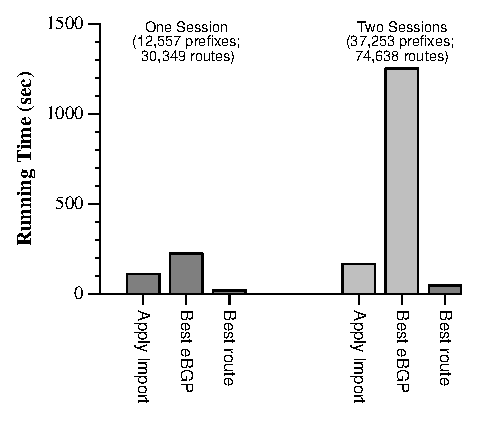
\epsfig{file=figures/peerperf.eps, height=1.75in, width=0.65\linewidth}
%% \caption{Performance of the emulator for a smaller number of eBGP sessions} 
%% \label{fig:peerperf}
%% \end{figure}


%\subsection{Computing the Set of Best eBGP Routes}

%% \begin{table}[t]
%% \begin{small}
%% \begin{center}
%% \begin{tabular}{r|r|r|r}
%% & {\em Predictions} & {\em Time (sec)} & {\em Prefixes/sec}\\ \hline
%% Without caching & 92419 & 17537 & 5.27 \\  \hline 
%% With caching & 8091 & 12033 & 8.23 \\
%% \end{tabular}
%% \end{center}
%% \end{small}
%% \caption{Running times for the second module, which
%%   computes the set of 
%%   best eBGP routes. Recognizing that prefixes can be grouped according
%%   to how they are advertised produces a significant speedup.  
%% }
%% \label{tab:perf2}
%% \end{table}

%
%However, recognizing that groups of prefixes are often advertised in
%exactly the same fashion allows the emulator to avoid recomputing the
%best routes for prefixes that are equivalent in terms of where they are
%advertised, the attributes they are advertised with, etc.  
%and subsequently performs route prediction by figuring out which group
%of equivalent prefixes a particular prefix belongs to.  Then, the module
%checks its cache to determine if it has already computed the set of best
%eBGP routes for some prefix in the group. In the case of a cache hit,
%the module simply reuses the previously computed answer; otherwise, it
%performs the prediction algorithm from Figure~\ref{fig:ep_pseudo}.


%% Figure~\ref{fig:peerperf} shows the running times for the second module
%% with one and two eBGP sessions and caching enabled.  The speedup for a
%% small number of sessions is not as dramatic as for other modules,
%% because, even for a small number of prefixes, there is not a linear
%% reduction in the number of prefixes and routes.  Nevertheless, the
%% running times are considerably smaller than for a network as large as
%% AT\&T's. 

%% \subsection{Computing the Best Route at Each Router}

%% \begin{table}[t]
%% \begin{small}
%% \begin{center}
%% \begin{tabular}{r|r|r|r|r}
%% & {\em Hits} & {\em Misses} & {\em Time (sec)} & {\em prefixes/sec}\\ \hline
%% Without caching & --- & --- & 390 & 211.6 \\ \hline 
%% With caching    & 82245 & 290 & 245 & 336.9 \\ 
%% \end{tabular}
%% \end{center}
%% \end{small} 
%% \caption{Running times and cache performance for the third module, which
%%   computes the best egress router. The results are 
%% from the validation of RR1, where predictions are made for 82,535
%% prefixes. This is one less than the 82,536 prefixes that we 
%% validated, as one prefix had an empty egress set (a Case 1 error for
%%   which we could not make a prediction).
%% }
%% \label{tab:perf3} 
%% \end{table}

%% Table~\ref{tab:perf3} shows the running time and cache performance for
%% the third module. The results come from the validation test of RR1
%% from Table~\ref{tab:predictions_summary}. The performance of the third
%% module is greatly improved by exploiting the nature of routing table
%% data.  For an ingress router, we only need to calculate the best
%% egress router for a given egress set once. Without caching, it takes
%% 390 seconds to predict the best egress router for the 82,535 prefixes
%% at this router, or about 212 prefixes per second. 

%Figure~\ref{fig:peerperf} shows that module 3's running time is
%comparatively small: 19 seconds and 47 seconds for one and two eBGP
%sessions, respectively. 

%%%
%%% validation.tex
%%%

\subsection{Validation}
\label{sec:validation}
%%%
%%% Approach
%%%
%Ensuring that the emulator produces correct answers is important
%because we envision operators using such a tool to evaluate potential
%configuration changes in an operational network.  
To verify that the emulator produces correct answers,
we perform 
validation using complete routing protocol implementations
on production routers in a large operational network.  
Network simulators do not capture the full
details of the standard routing protocols, so it is not useful to
compare the emulator's results with those of a simulator.  
In addition, we may be 
unaware of vendor-specific variations that could affect the accuracy
of our results.  Since we cannot make arbitrary changes to deployed
configurations on a live network,
we run the emulator on individual snapshots derived from daily
dumps of the router configuration files, BGP routing tables, and BGP 
neighbor information and compare the emulator's route predictions to
what was seen in practice.  For each phase of the algorithm, we compare 
our results to actual BGP tables and present a breakdown of any 
mismatches we encounter.  To isolate the sources of inaccuracy, we 
evaluate each phase in Figure~\ref{fig:dataflow} independently, assuming
perfect inputs from  
the previous module; we also perform an end-to-end validation.

The emulator generates correct results for more than $99\%$ of the 
prefixes. Most mismatches can be attributed to the fact
the data sets were collected at slightly different times.
%This problem is unavoidable since process of ``dumping''
%the network state occurs over a period of several hours, as polling
%engines contact each router and download large quantities of data.
%Inevitably, the network state will change during this period.
%These inconsistencies are rare and do not significantly 
%influence the accuracy of the emulation.
%%%
%%% Data
%%%
The analysis focuses on a snapshot of the network state from early
morning (EST) on February 4, 2003.  We validate the prediction algorithm
for the 91,554
prefixes whose eBGP routes are
learned at peering points to other large providers, since we have routing
tables from all of these locations; we
excluded prefixes that were learned at other routers.
% for which we did not have routing
%tables, such as customer routers. 
%We focus
%on these prefixes because we have routing tables for every router that
%advertises these prefixes 
(Recall that the prediction algorithm relies
on knowing all of the potential egress routers where routes to a prefix
are learned.)
%We expect the results for the prefixes that we have excluded to be
%comparable to those that we are able to validate. 
%That is, we exclude the routes learned from customers and instead
%focus on the routing of outbound traffic to the rest of the Internet.
The initial BGP routing data consists of 1,620,061 eBGP-learned routes
with 43,434 distinct AS paths.  We applied the tool
to these inputs and checked whether the emulator produced the same
answers that the operational routers selected.  In addition to
collecting BGP routing tables from the peering routers (where the eBGP
routes are learned), we also collected BGP tables from several 
route reflectors and access routers to verify the results.

\subsubsection{Applying Import Policy}
To verify that the first phase correctly emulates the application of
import policy, we need only compare the route attributes (\ie, local
preference, MED, etc.) in the {\dfc modified routes} table to the
actual BGP routing tables.  The {\dfc modified routes} table contains
the routes with attributes modified by applying the import policies
specified in the {\mf import} table to the initial {\mf known routes}
table.  Because the prototype uses routing tables to approximate the
actual routes received at each router in the AS, we cannot
determine what routes were discarded by the import policy.  Thus, the
emulator cannot emulate the filtering policies specified by import
policies, but it can still determine the
effects of import policy configurations that set or manipulate 
route attributes (\eg, for traffic engineering).
%The {\mf known routes} table contains only the eBGP-learned routes,
%since subsequent modules emulate the behavior of iBGP.  In addition,
%our analysis excludes the routes learned from customers since we
%analyze data collected from the peering points.
%J We can skip this point
%we have Because subsequent modules emulate the behavior of iBGP, we do not need
%to incorporate iBGP-learned routes.  The emulator could incorporate
%customer routes, but we choose not to do so: because networks typically
%(1) always prefer sending traffic through customers and (2) accept
%whatever route attributes accompany the customer's route advertisements,
%it is not reasonable to change import policy to affect traffic flow on
%these routes.
%

\begin{table}
\begin{center}
{\small
\begin{tabular}{r|r|p{0.825in}p{0.825in}|l}
& {\em Number} & \parbox{0.825in}{{\em Attribute \\ Mismatch}} &
  \parbox{0.825in}{{\em Unusual\\ Configuration}} & {\em Total Errors}
  \\ \hline 
%Routers & 2 & 2 & 4 & 28.57\% (4/14) \\ \hline
AS Paths & 43,434 & 3 & 9 & 12 (0.028\%) \\ %\hline
Routes & 1,620,061 & 36 & 277 & 313 (0.019\%) \\ %\hline
\end{tabular}
\vspace{-0.15in}
}
\end{center}
\caption{Summary of errors in applying import policy.  
%Most of the errors
%  resulted from the fact that the prototype implementation does not
%  currently handle a special configuration case.
}
\label{tab:mismatch_summary}
\end{table}

We compared the route attributes between the {\mfc known routes} and
{\mfc modified routes} tables for all 1,620,061 eBGP routes
with 43,434 distinct AS paths.
% from 14 peering routers.  
Table~\ref{tab:mismatch_summary} summarizes the results of our
validation.  The emulator's results matched the route attributes seen in
the BGP tables for all but 313 eBGP-learned routes on 
12 distinct AS paths.  We observed 36 attribute mismatches over 3 AS
paths, which can likely be attributed to actual policy changes, since
the routing tables and the configuration files were captured at
slightly different times of day; we verified this conclusion by
inspecting the configuration data for the next day.  The remaining
mismatches involved 9 unique AS paths because the prototype did not
handle a complex configuration scenario permitted on Cisco routers.
% (one route map used a \texttt{deny} statement when
%in its \texttt{as-path access-list} statement, which the current
% implementation of our prototype does not parse).  
This accounted for 277 of the 313 route mismatches.
Overall, the first phase produced successful results for more than
99.97\% of the cases. 

%This high success rate is expected: the only time we would expect to see
%a mismatch between the emulation and the actual observed local
%preference values would be if router configuration had changed between
%the capture of the configuration file and the capture of the BGP table.

\subsubsection{Computing the Set of Best eBGP Routes}


\begin{table}
\begin{center}
{\small
\begin{tabular}{r|r|rr|l}
& {\em Number} & {\em Different} & {\em Missing} & {\em Total Errors}\\ \hline 
AS Paths & 43,434 & 66 & 187 & 253 (0.582\%) \\ %\hline %/45922 
Prefixes & 91,554 & 120 & 483 & 603 (0.659\%) \\ %\hline %/92348
\end{tabular}
\vspace{-0.15in}
}
\end{center}
\caption{Mispredictions in the set of best eBGP routes.
%  at network exit points.
%  The table shows the number of best eBGP route predictions
%  that did not agree with the route chosen by the corresponding route
%  reflector.
%  Most of the errors resulted from timing inconsistencies: instances
%  where the BGP emulator predicted a route for a prefix that did not
%  exist in the route reflector tables.
} 
\label{tab:mismatch_summary_box2}
\end{table}

%As discussed in Section~\ref{sec:best_exit}, the module that computes
%the best routes at network exist points computes a function that maps a
%prefix to a set of possible egress points (\ie, next-hop IP addresses),
%where each egress point corresponds to some route heard at one of the
%domain's border routers.  To validate this computation, we must
%determine whether the best route that this module has predicted at the
%network exit point is the same as the best route that was actually
%selected at that network exit point.  

%To validate the computation of the set of best eBGP routes, 
%we compare
%the results 
%of the second module with the best routes selected at each top-level
%route reflector in the operational network. 
%To verify that the best eBGP routes computed by the emulator were the
%same as those computed as the actual set of best eBGP routes, we
%compared each route in the set of best eBGP routes with the
%corresponding routing table entry at the nearest RR.  
To verify that the second phase correctly computes the set of best eBGP
routes, 
we check that the best route at each eBGP-speaking router as specified by
the {\dfc egress points} table corresponds to the route that appears in
the routing table of that router's route reflectors. 
These routes
match the vast majority of the time.  However, in a few cases, the two
routers had different routes (\ie, with different AS paths), even
though one router apparently learned the route directly from the
other; these results are summarized in the ``Different'' column in
Table~\ref{tab:mismatch_summary_box2}.  The ``Missing'' column
highlights cases where the route reflector did not have {\em any\/}
route for that 
prefix.  Timing inconsistencies can explain both scenarios, which
together account for just over 0.5\% of the cases.

%Next, we checked that each RR selected a best route that appeared in
%the set of best eBGP routes by the emulator.  
To verify that the emulator does not incorrectly exclude routes from the
set of best eBGP routes, we check that, for each prefix, the best route
at each route reflector appears in the set of best eBGP routes as computed by
the emulator\footnote{The reverse is not necessarily true.  An
egress point may have a larger IGP path cost to each
of the top-level route reflectors for certain sets of eBGP routes.}.
In other words, we consider
cases where a route reflector's best route would have directed traffic towards
some egress router that was not contained in the {\dfc egress points}
table.  Only 1.11\% of best routes at route reflectors 
% (4,945 of 1,295,009 best routes) 
% (14,480 of 1,295,009 best routes) 
% (4,945 of 1,295,009 best routes) 
for 2\% of prefixes 
%(1,871 of 91,554 prefixes) 
%(1,216 of 91,252 prefixes)  --old
fell into this category.  %Examination of these anomalies suggests that
Routing dynamics can explain these inconsistencies---through
manual inspection, we found that, in many cases, the best route at the
RR was clearly worse than the routes in the set of best eBGP routes
(\eg, the route reflector's best route had the same local preference but a higher
AS path length).  
%Often, the corresponding egress router's BGP table
%had a different route (\eg, with a higher local preference, shorter
%AS path, etc.).
%, consistent with the ``Different'' case in
%Table~\ref{tab:mismatch_summary_box2}.

\subsubsection{Computing the Best Route at Each Router}

%In this section, we describe the validation of the third module, which
%computes the best egress router, given an ingress router and a
%destination prefix. We also discuss mispredictions made by the
%third module, and account for these errors.

To verify that the emulator correctly predicts the best egress
router, we examined the best routes in BGP tables at several routers and
compared the (destination prefix, 
next-hop) pair from the routing table with the results in the {\df
predicted routes} table entry for that router.  
%We performed these comparisons at four different routers in the network.
We performed these comparisons at two
access routers that connected directly to
customers in different 
geographic locations
to verify that the emulator makes correct predictions at ingress
routers.  We also analyzed the emulator's predictions at two route
reflectors to verify that the algorithm makes correct route predictions
as it traverses the signaling graph.
%
%The routing tables we use for verification are collected from route
%reflectors and access routers within the AT\&T network. While access
%routers, which receive traffic entering the network from customers,
%are clearly ingress routers, this classification does not quite fit
%for route reflectors. Though not a ingress router, a route reflector
%serves the same value for validation as the access routers. Recall
%that we are focusing on prefixes advertised to AT\&T on eBGP sessions
%with peering ASes. As route reflectors and access routers are internal
%to the network, their best next hop for these external prefixes, will
%be the AT\&T eBGP router that learned of the prefix from the peer
%AS. The advertisements for these prefixes are propagated through iBGP
%sessions from the eBGP router to internal routers, such as route
%reflectors and access routers. The routing tables of these two types
%of routers are therefore perfect candidates for validating the third
%module, as they will test that the module correctly emulates the
%interaction between eBGP learned routes, and the iBGP topology and IGP
%configuration.
The best route matched our prediction for 99.5-99.7\% of the cases, as
summarized in Table~\ref{tab:predictions_summary}.  At each router, 
we excluded prefixes if the best egress router was not one of
the peering routers included in the {\mfc known routes} table (recall
that we excluded routers for which we did not have routing tables%, such
%as customer routers
). In these cases, we cannot evaluate whether the
algorithm would have made the correct prediction because we didn't
have the routes from that egress router in the first place.

%{\em Case 1:} The destination prefix at the ingress router does not
%  appear in the {\df known routes} table, causing the emulator to
%  predict an empty egress set. 


We classify the
errors among the remaining prefixes in terms of three cases:
%We have classified the mismatches into four cases, where the first three 
%described below. The first three cases directly show that the error
%resulted from timing inconsistencies between routing table data. This
%is likely the explanation for the errors in case 4 as well. 
{\em Case 1:} The route at the ingress router does not appear in
  the {\dfc modified routes} table and, as such, does not appear in the
  egress set. 
{\em Case 2:} The route at the ingress router appears in the
  {\dfc modified routes} table but does not appear in the {\dfc egress
    points} table.  
{\em Case 3:} The misprediction has no obvious explanation.
%Other misprediction. Again, these errors are likely
%caused by the variable nature of BGP routing state in the network. For
%example, the best egress router predicted by the emulator, may have
%been unavailable to the router being validated, due to a route withdrawal.

Case 1 errors likely result from timing inconsistencies, where the best
route at the ingress router did not exist at the egress router when the
routing tables were dumped.  Timing inconsistencies can also explain
Case 2 errors: for example, an ingress router or a route reflector could
have a route that is no longer one of the best eBGP-learned routes, which
could happen if a better route arrived at an eBGP-speaking router but
had not yet propagated to other routers in the AS.  We are unable to
explain only 0.05\% of the errors.

\begin{table}
\begin{center}
{\small
\begin{tabular}{r|r|rrr|l}
{\em Router} & {\em \# Predictions}
& {\em Case 1} & {\em Case 2}
& {\em Case 3} & {\em Total Errors} \\ \hline 

RR1 &   88,865&  33&  322& 21 &  376 (0.423\%)   \\ %\hline
RR2 &   88,164&  33&  185&  5 &  223 (0.253\%)   \\ %\hline
AR1 &   88,165&  38&  178&  5 &  221 (0.251\%)    \\ %\hline
AR2 &   76,547& 151&  170& 37 &  358 (0.468\%)   \\ %\hline
\end{tabular}
\vspace{-0.15in}
}
\end{center}
\caption{Errors in predicting the best egress router.
  Prefixes predicted incorrectly by the second phase and those where
  the ``right'' answer was not a peering router are excluded.
%from inside the network. 
%Shown are the number of predictions that do not
%correspond to the best egress router from the BGP routing table. 
%The 603
%prefixes that were incorrectly predicted by the second module are
%excluded.  XXX Fix this table and discussion. XXX
%Cases
%1-3 result from timing inconsistencies. Errors in case 4 may also relate 
%to inconsistent data.
} 
\label{tab:predictions_summary}
\end{table}

\subsubsection{End-to-End Validation}
\begin{table}
\begin{center}

{\small
\begin{tabular}{r|r|rrr|l}
{\em Router} & {\em \# Predictions}
& {\em Case 1} & {\em Case 2}
& {\em Case 3} & {\em Total Errors} \\ \hline 

RR1 &   89,343&  40&  459& 55 &  554 (0.620\%)   \\ %\hline
RR2 &   88,647&  39&  314& 41 &  394 (0.444\%)   \\ %\hline
AR1 &   88,649&  44&  307& 40 &  391 (0.441\%)    \\% \hline
AR2 &   76,733& 157&  283& 71 &  511 (0.666\%)   \\ %\hline
\end{tabular}
\vspace{-0.15in}
}
\end{center}
\caption{Summary of errors for end-to-end validation.} 
\label{tab:e2e_summary}
\end{table}

We performed an end-to-end validation to study the effect of error
propagation on the best routes ultimately predicted by the emulator.
We compared the emulator's prediction with the same four routing
tables used for the validation of the third module, with the exception
that the input included the errors from the first two modules.  At
these four routers, the emulator predicted the correct routes for more
than 99\% of all prefixes, as summarized in Table~\ref{tab:e2e_summary}.
%
We hypothesized that the majority of the mispredicted routes could be
explained by the dynamics of the input data.  
%A modification to the import policy could have changed the choice of
%best route between the time the two routing tables were captured.  A
%more likely explanation is that the inconsistencies were caused by
%routing dynamics that caused the temporary appearance or disappearance
%of a route.
For example, if the best route at an eBGP-speaking router were
temporarily withdrawn at the time that the route reflector table was
captured, inconsistencies between routing tables could
arise\footnote{To evaluate our hypothesis, we analyzed a feed of iBGP
update messages collected on the same day.  More than 45\% of the
prefixes with incorrect predictions had a BGP routing change during
the data collection period at the same router where the apparent
mismatch occurred, and 83\% of the prefixes experienced an update at
some router in the AS during this period.}.
%Would be good to report the percent of *all* prefixes
%that had an update during that period, to illustrate that the
%mismatches are unusual in terms of having more updates (assuming that
%this is true).

These results suggest that the algorithm we have proposed is accurate:
prediction errors are infrequent and result mainly 
the dynamics of the inputs.  Since most prefixes whose routes change
frequently do not receive much traffic~\cite{Rexford:stability2002}, these
inconsistencies would certainly not prevent the emulator from
being used for traffic engineering tasks.
%Ideally, the emulator would receive a real-time stream of all of the
%eBGP-learned routes.  However, this is not currently possible because
%commercial routers only support either (1)~dumping the entire BGP
%table (which contains all of the routes after import processing, but
%imposes a load on the router and provides only a static view) or
%(2)~having a BGP session to a monitor (which provides a real-time view
%of only the current best routes after import processing).












%% \subsubsection{Performance evaluation}

%% We ran the prototype on a Sun Fire 15000 with 192 GB of RAM and 48
%% 900 MHz Ultrasparc-III Copper processors.  Because this is a time-shared
%% machine, we ran each of our experiments several times to ensure the
%% accuracy of our measurements.  Except where noted, the prototype used
%% only two 900 MHz processors (one for the database process and one for
%% the emulator itself); the combined memory footprint of the
%% database process and the emulator never exceeded 50 MB.  Because the
%% emulator did not use more resources than a standard PC, the results of
%% our evaluation should reasonably reflect the emulator's
%% performance on commodity hardware.


%% While our evaluation is preliminary, our performance tests demonstrate
%% that the prototype can operate on timescales that could allow an operator
%% to use a BGP prototype based on our algorithms in a practical setting.
%% Our evaluation demonstrates the following points:
%% \begin{itemize}
%% \itemsep=-1pt
%% \item The prototype computes the best routes for {\em one prefix\/} throughout a
%%   large tier-1 ISP network in about one second.  Although predicting the
%%   best route for {\em all\/} prefixes at all routers in such a
%%   network takes several hours, this type of computation does not need to
%%   be performed all that frequently in practice.
%% \item Exploiting commonalities among route advertisements
%%   to eliminate redundant computation reduces
%%   the running time of the prototype by approximately 50\%.
%% \item Evaluating the effects of an incremental
%%   change to router configuration typically takes only a few seconds.
%% \end{itemize}


%% \subsubsection{Validation}

%% To verify that the prototype produces correct answers, we perform
%% validation using complete routing protocol implementations on production
%% routers in a large operational network.  We performed independent
%% validation for each of the three modules, as well as 
%% an end-to-end validation to study the effect of error
%% propagation on the best routes ultimately predicted by the prototype.
%% We summarize the results of the end-to-end
%% evaluation here. 

%% We compared the prototype's computation with the same four routing
%% tables used for the validation of the third module, with the exception
%% that the input included the errors from the first two modules.  At
%% these four routers, the prototype predicted the correct routes for more
%% than 99\% of all prefixes, as summarized in Table~\ref{tab:e2e_summary}.
%% \begin{table}[h!]
%% \begin{center}
%% {\small
%% \begin{tabular}{r|r|l}
%% {\em Router} & {\em \# Predictions} & {\em Total Errors} \\ \hline 

%% RR1 &   89,343&  554 (0.620\%)   \\ %\hline
%% RR2 &   88,647&  394 (0.444\%)   \\ %\hline
%% AR1 &   88,649&  391 (0.441\%)    \\% \hline
%% AR2 &   76,733&  511 (0.666\%)   \\ %\hline
%% \end{tabular}
%% \vspace{-0.15in}
%% }
%% \end{center}
%% \caption{Summary of errors for end-to-end validation.} 
%% \label{tab:e2e_summary}
%% \end{table}
%% Prediction errors are infrequent and result mainly the dynamics of the
%% inputs.  Since most prefixes whose routes change frequently do not
%% receive much traffic~\cite{Rexford:stability2002}, these inconsistencies would
%% be permissible for most traffic
%% engineering tasks.
